% ------------------------------------------------------------------------------
% TYPO3 Version 10.3 - What's New (English Version)
%
% @author	Michael Schams <schams.net>
% @license	Creative Commons BY-NC-SA 3.0
% @link		https://typo3.org/help/documentation/whats-new/
% @language	English
% ------------------------------------------------------------------------------

\section{Changes for Developers}
\begin{frame}[fragile]
	\frametitle{Changes for Developers}

	\begin{center}\huge{Chapter 3:}\end{center}
	\begin{center}\huge{\color{typo3darkgrey}\textbf{Changes for Developers}}\end{center}

\end{frame}

% ------------------------------------------------------------------------------
% Feature | 90333 | Dashboard

\begin{frame}[fragile]
	\frametitle{Changes for Developers}
	\framesubtitle{Dashboard (1)}

	% decrease font size for code listing
	\lstset{basicstyle=\smaller\ttfamily}

	\begin{itemize}
		\item Developers can create custom widgets for the Dashboard by extending one of the following widget \textit{abstracts}:

			\begin{itemize}
				\item \texttt{AbstractWidget}\newline
					\small
						A basic abstract that can be used as the start of simple widgets.
					\normalsize
				\item \texttt{AbstractRssWidget}\newline
					\small
						An abstract to create a widget that shows a RSS feed.
					\normalsize
				\item \texttt{AbstractListWidget}\newline
					\small
						An abstract to create a widget that shows a list of items.
					\normalsize
				\item \texttt{AbstractCtaButtonWidget}\newline
					\small
						An abstract to create a widget that shows a "call-to-action" button.
					\normalsize
			\end{itemize}

	\end{itemize}

\end{frame}

% ------------------------------------------------------------------------------
% Feature | 90333 | Dashboard

\begin{frame}[fragile]
	\frametitle{Changes for Developers}
	\framesubtitle{Dashboard (2)}

	% decrease font size for code listing
	\lstset{basicstyle=\tiny\ttfamily}

	\begin{itemize}
		\item Register your widgets in the following file of your extension:\newline
			\texttt{EXT:my\_extension/Configuration/Services.yaml}

		\item Option 1: widget identifier as attribute

\vspace{-0.4cm}
\begin{lstlisting}
Vendor\MyExtension\Widgets\MyFirstWidget:
  tags:
    - name: dashboard.widget
      identifier: widget-identifier-1
      widgetGroups: 'general'
\end{lstlisting}

		\item Option 2: custom service name allows multiple widget identifier to share one class

\vspace{-0.4cm}
\begin{lstlisting}
widget.identifier:
  class: Vendor\MyExtension\Widgets\MySecondWidget
  tags:
    - name: dashboard.widget
      identifier: widget-identifier-2
      widgetGroups: 'general, typo3'
\end{lstlisting}

	\end{itemize}

\end{frame}

% ------------------------------------------------------------------------------
% Feature | 90333 | Dashboard

\begin{frame}[fragile]
	\frametitle{Changes for Developers}
	\framesubtitle{Dashboard (3)}

	% decrease font size for code listing
	\lstset{basicstyle=\tiny\ttfamily}

	\begin{itemize}
		\item Every widget is attached to one or more widget groups.
		\item Those groups are shown in the modal when adding a new widget to your dashboard.
		\item Developers can configure custom widget groups by creating a file\newline
			\smaller
				\texttt{EXT:my\_extension/Configuration/Backend/DashboardWidgetGroups.php}
			\normalsize

\vspace{-0.4cm}
\begin{lstlisting}
return [
  'widgetGroup-exampleGroup' => [
    'title' => 'LLL:EXT:my_extension/Resources/Private/Language/locallang.xlf:widget_group_name',
  ],
];
\end{lstlisting}

	\end{itemize}

\end{frame}

% ------------------------------------------------------------------------------
% Feature | 89870 | New PSR-14 Events for Extbase-related signals

\begin{frame}[fragile]
	\frametitle{Changes for Developers}
	\framesubtitle{Extbase and Fluid}

	% decrease font size for code listing
	\lstset{basicstyle=\tiny\ttfamily}

	\begin{itemize}
		\item The following PSR-14-based events have been introduced for Extbase-related signals:

\vspace{-0.4cm}
\begin{lstlisting}
TYPO3\CMS\Extbase\Event\Mvc\AfterRequestDispatchedEvent
TYPO3\CMS\Extbase\Event\Mvc\BeforeActionCallEvent
TYPO3\CMS\Extbase\Event\Persistence\AfterObjectThawedEvent
TYPO3\CMS\Extbase\Event\Persistence\ModifyQueryBeforeFetchingObjectDataEvent
TYPO3\CMS\Extbase\Event\Persistence\ModifyResultAfterFetchingObjectDataEvent
TYPO3\CMS\Extbase\Event\Persistence\EntityAddedToPersistenceEvent
TYPO3\CMS\Extbase\Event\Persistence\EntityFinalizedAfterPersistenceEvent
TYPO3\CMS\Extbase\Event\Persistence\EntityUpdatedInPersistenceEvent
TYPO3\CMS\Extbase\Event\Persistence\EntityRemovedFromPersistenceEvent
TYPO3\CMS\Extbase\Event\Persistence\EntityPersistedEvent
\end{lstlisting}

		\item Existing signals have been replaced and should not be used anymore.

	\end{itemize}

\end{frame}

% ------------------------------------------------------------------------------
% Feature | 89644 | Add optional argument fields to editRecord ViewHelpers

\begin{frame}[fragile]
	\frametitle{Changes for Developers}
	\framesubtitle{ViewHelper \texttt{editRecord}}

	% decrease font size for code listing
	\lstset{basicstyle=\tiny\ttfamily}

	\begin{itemize}
		\item An optional argument \texttt{fields} has been added to the
			\texttt{uri.editRecord} and \texttt{link.editRecord} ViewHelpers.
		\item If set, the FormEngine creates a form to only edit the given database field(s).
		\item The following example creates a link to edit the \texttt{tt\_content.bodytext}
			field of record with the UID 42.

\begin{lstlisting}
<be:link.editRecord uid="42" table="tt_content" fields="bodytext" returnUrl="foo/bar">
  Edit record
</be:link.editRecord>
\end{lstlisting}

	\end{itemize}

\end{frame}

% ------------------------------------------------------------------------------
% Feature | xxxxx | Introduce AssetCollector

\begin{frame}[fragile]
	\frametitle{Changes for Developers}
	\framesubtitle{AssetCollector}

	\begin{itemize}
		\item The initial steps of integrating an AssetCollector have been implemented.
		\item The concept allows developers to add custom CSS/JS code (inline or external)
			multiple times, but TYPO3 outputs it only once.
		\item In this regards, two new Fluid ViewHelpers have been added:
			\begin{itemize}
				\item \texttt{<f:asset.css>}
				\item \texttt{<f:asset.script>}
			\end{itemize}
		\item In the long run, the AssetCollector aims to replace the various existing
			TypoScript options that are rather confusing.
	\end{itemize}

\end{frame}

% ------------------------------------------------------------------------------
% Feature | 86614 | Add PSR-14 event to control hreflang tags to be rendered

\begin{frame}[fragile]
	\frametitle{Changes for Developers}
	\framesubtitle{Modify \texttt{hreflang}-tag}

	% decrease font size for code listing
	\lstset{basicstyle=\smaller\ttfamily}

	\begin{itemize}
		\item It is now possible to modify \texttt{hreflang} tags before they get rendered.
		\item Developers can achieve this by registering an event listener for the following event:\newline
			\smaller
				\texttt{TYPO3\textbackslash
					CMS\textbackslash
					Frontend\textbackslash
					Event\textbackslash
					ModifyHrefLangTagsEvent}
			\normalsize
	\end{itemize}

\end{frame}

% ------------------------------------------------------------------------------
% Feature | 88818 | Introduce events to modify CKEditor configuration

\begin{frame}[fragile]
	\frametitle{Changes for Developers}
	\framesubtitle{Modify the CKEditor Configuration}

	% decrease font size for code listing
	\lstset{basicstyle=\tiny\ttfamily}

	\begin{itemize}
		\item The following PSR-14-based events have been introduced which allow to modify the CKEditor configuration:

\vspace{-0.4cm}
\begin{lstlisting}
TYPO3\CMS\RteCKEditor\Form\Element\Event\AfterGetExternalPluginsEvent
TYPO3\CMS\RteCKEditor\Form\Element\Event\BeforeGetExternalPluginsEvent
TYPO3\CMS\RteCKEditor\Form\Element\Event\AfterPrepareConfigurationForEditorEvent
TYPO3\CMS\RteCKEditor\Form\Element\Event\BeforePrepareConfigurationForEditorEvent
\end{lstlisting}

		\item The
			\href{https://docs.typo3.org/c/typo3/cms-core/master/en-us/Changelog/10.3/Feature-88818-IntroduceEventsToModifyCKEditorConfiguration.html}{change log}
			for an example.
	\end{itemize}

\end{frame}

% ------------------------------------------------------------------------------
% Feature | 90265 | Show dispatched Events in Admin Panel

\begin{frame}[fragile]
	\frametitle{Changes for Developers}
	\framesubtitle{PSR-14 Events in Admin Panel}

	\begin{itemize}
		\item The Admin Panel shows all PSR-14 events that have been dispatched in the current request.
	\end{itemize}

	\begin{figure}
		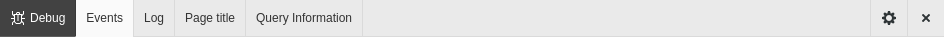
\includegraphics[width=0.85\linewidth]{ChangesForDevelopers/90265-ShowDispatchedEventsInAdminPanel.png}
	\end{figure}

\end{frame}

% ------------------------------------------------------------------------------
% Feature | 89738 | API for AJAX Requests

\begin{frame}[fragile]
	\frametitle{Changes for Developers}
	\framesubtitle{API for AJAX Requests}

	% decrease font size for code listing
	\lstset{basicstyle=\tiny\ttfamily}

	\begin{itemize}
		\item The \textbf{Fetch API} has been introduced to perform AJAX requests
			and to make TYPO3 less dependent on jQuery.
		\item The API provides a generic definition of Request and Response objects
			(and other things involved with network requests).
		\item Supported by all modern browsers, see
			\href{https://developer.mozilla.org/en-US/docs/Web/API/Fetch_API}{compatibility chart}.
		\item The TYPO3 core uses the new API in the Install Tool, FormEngine, and
			context menus already.
		\item See the
			\href{https://docs.typo3.org/c/typo3/cms-core/master/en-us/Changelog/10.3/Feature-89738-ApiForAjaxRequests.html}{change log}
			for some examples on how to use the Fetch API.

	\end{itemize}

\end{frame}

% ------------------------------------------------------------------------------
% Feature | 89650 | Allow line breaks in TCA descriptions

\begin{frame}[fragile]
	\frametitle{Changes for Developers}
	\framesubtitle{TCA Description Fields}

	\begin{itemize}
		\item The description field in the TCA can now contain line breaks to make long texts more readable.
	\end{itemize}

\end{frame}

% ------------------------------------------------------------------------------
% Important | 90020 | Legacy BasicFileUtility and ExtendedFileUtility classes marked as internal

\begin{frame}[fragile]
	\frametitle{Changes for Developers}
	\framesubtitle{Classes \texttt{BasicFileUtility} and \texttt{ExtendedFileUtility}}

	\begin{itemize}
		\item The following two legacy classes have been marked as \textbf{internal}
			and should not be used anymore:

			\begin{itemize}\small
				\item \texttt{TYPO3\textbackslash
					CMS\textbackslash
					Core\textbackslash
					Utility\textbackslash
					File\textbackslash
					BasicFileUtility}
				\item \texttt{TYPO3\textbackslash
					CMS\textbackslash
					Core\textbackslash
					Utility\textbackslash
					File\textbackslash
					ExtendedFileUtility}
			\end{itemize}

		\item Extension developers should use the classes \texttt{ResourceStorage}
			and \texttt{ResourceFactory} for managing assets instead.

	\end{itemize}

\end{frame}

% ------------------------------------------------------------------------------
% Feature | 89139 | Add dependency injection support for console commands

\begin{frame}[fragile]
	\frametitle{Changes for Developers}
	\framesubtitle{Console Commands: Symfony DI Support}

	\begin{itemize}
		\item Command dependencies can now be injected via constructor or other injection techniques.
		\item Add the \texttt{console.command} tag to command classes.
		\item Use the tag attribute \texttt{command} to specify the command name.
		\item The optional tag attribute \texttt{schedulable} can be set to \texttt{false}
			to exclude the command from the TYPO3 scheduler.

		\item See
			\href{https://docs.typo3.org/c/typo3/cms-core/master/en-us/Changelog/10.3/Feature-89139-AddDependencyInjectionSupportForConsoleCommands.html}{change log}
			for an example.
	\end{itemize}

\end{frame}

% ------------------------------------------------------------------------------
% Feature | 90168 | Introduce Modal Actions

\begin{frame}[fragile]
	\frametitle{Changes for Developers}
	\framesubtitle{Action Buttons in Modals}

	% decrease font size for code listing
	\lstset{basicstyle=\tiny\ttfamily}

	\begin{itemize}
		\item Modal popups now support action buttons.
		\item As an alternative to the existing \texttt{trigger} option, the new option
			\texttt{action} can be used.
		\item For example:

\vspace{-0.4cm}
\begin{lstlisting}
Modal.confirm('Header', 'Some content', Severity.error, [
  {
    text: 'Based on trigger()',
    trigger: function () {
      console.log('Vintage!');
    }
  },
  {
    text: 'Based on action()',
    action: new DeferredAction(() => {
      return new AjaxRequest('/any/endpoint').post({});
    })
  }
]);
\end{lstlisting}

	\end{itemize}

\end{frame}

% ------------------------------------------------------------------------------
% Feature | 90471 | JavaScript Event API

\begin{frame}[fragile]
	\frametitle{Changes for Developers}
	\framesubtitle{JavaScript Event API}

	\begin{itemize}
		\item A new Event API enables JavaScript developers to have a stable event listening interface.
		\item The API takes care of common pitfalls like event delegation and clean event unbinding.
		\item Each \textit{event strategy} offers two ways to bind a listener to an event.
		\item The Event API offers several strategies to handle event listeners.
		\item See
			\href{https://docs.typo3.org/c/typo3/cms-core/master/en-us/Changelog/10.3/Feature-90471-JavaScriptEventAPI.html}{change log}
			for examples and further details.
	\end{itemize}

\end{frame}

% ------------------------------------------------------------------------------
